\chapter{Processing Transient Alerts}
\label{chap:alerts}
\chaptoc{}

% ########################################

\newpage
\section{Introduction}
\label{sec:alerts_intro}
\begin{colsection}

In this chapter I describe the software used by GOTO to process alerts generated from transient astronomical events, including as gravitational wave detections.
%
\begin{itemize}
    \item In \nref{sec:alert_standards} I give an overview of the systems in place to publish and distribute astronomical alerts used by the LVC, NASA and other organisations.
    \item In \nref{sec:gotoalert} I describe the GOTO-alert Python module, which includes processing transient alerts, determining the optimal follow-up strategy and preparing targets for GOTO to observe.
\end{itemize}
%
All work described in this chapter is my own, and has not been published anywhere else.

\end{colsection}

% ########################################

\newpage
\section{Standards for reporting transient events}
\label{sec:alert_standards}
\begin{colsection}

% ~~~~~~~~~~~~~~~~~~~~

\begin{colsection}

\todo{Need to write little intro paragraph}

\end{colsection}

% ~~~~~~~~~~~~~~~~~~~~

\subsection{Transient astronomy}
\label{sec:transient_astronomy}
\begin{colsection}

\todo{This whole section needs adjusting}

For the last few decades the number of detections of transient astronomical sources has been rapidly increasing. From space-based gamma-ray burst monitors such as \textit{Fermi} and \textit{Swift} to wide-field survey telescopes such as the \gls{ptf} or \gls{asassn}, increasing numbers of time-critical events have been detected and therefore had to be rapidly sent to other observing partners for follow-up campaigns. Historically this was done, at a much slower pace, through physical post and telegrams --- hence the names of some of the current services offering modern, email-based alternatives: the Astronomer's Telegram \citep{ATel} GCN Circulars \citep{GCN}.

Today the global system has evolved to increasingly remove the human factor entirely in order to reduce the delay between events being detected and telescope observations being triggered. Robotic telescopes are now common and can be triggered automatically by machine processing of alerts generated automatically by the detection instruments. The \gls{ivoa} VOEvent protocol for transient alerts has become the standard language for such inter-robotic communications \citep{voevent}, allowing telescopes around to world to respond within seconds to transient alerts. Even then new projects such as the \gls{ztf}, itself paving the way for the imminent addition of the \gls{lsst}, will produce millions ove events per night requiring even faster and more efficient systems \citep{ZTF_alerts}.

GOTO's priority is of course detecting optical counterparts to gravitational wave events. Such events are published by the LIGO-Virgo Collaboration as VOEvents through the GCN Notice system, and the G-TeCS sentinel (see \aref{sec:sentinel}) is the system in charge of listening for and acting on those events when they occur, adding new pointings to the observation database to trigger the counterpart search.

In order for the \gls{goto} imaging pipeline to identify new sources that might be related to a gravitational wave signal it needs previous observations of the same point in the sky to compare to. Therefore for a majority of the time \gls{goto} observes an all-sky survey corresponding to a fixed grid, to build up an archive of reference images. Then as new exposures are taken they can be compared to these references, allowing new sources to be detected through difference imaging (see \aref{fig:difference_imaging}).

\begin{figure}[t]
    \begin{center}
        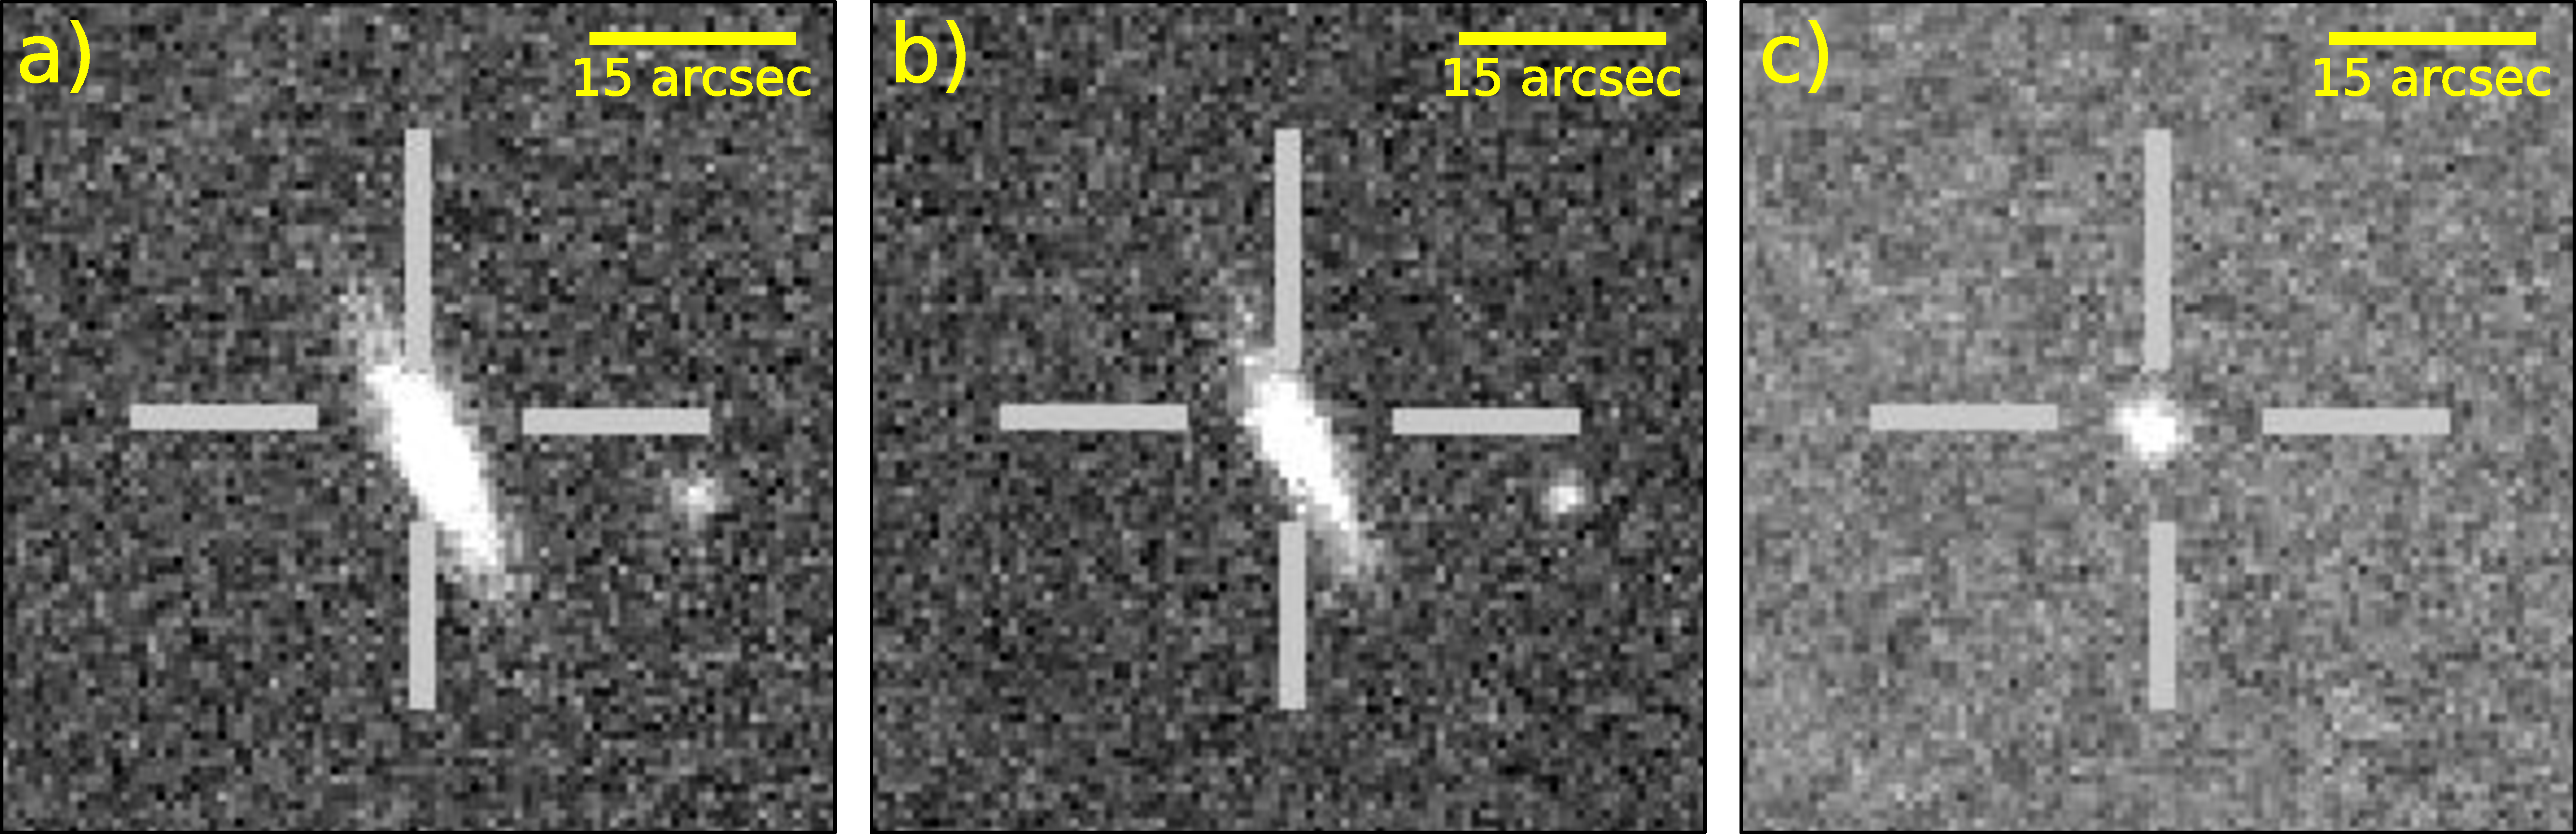
\includegraphics[width=\linewidth]{images/diffimg.pdf}
    \end{center}
    \caption[The detection of SN 2019bpc through difference imaging]{
        The detection of Type Ia supernova SN 2019bpc by the GOTOphoto difference imaging pipeline. The new exposure on the left (a) has the reference image (b) subtracted to give the difference image on the right (c), where the new source is clearly visible.
    }\label{fig:difference_imaging}
\end{figure}

\end{colsection}

% ~~~~~~~~~~~~~~~~~~~~

\subsection{GCN alerts}
\label{sec:gcn}
\begin{colsection}

The \gls{gcn}, also known as the Transient Astronomy Network or together GCN/TAN, is a system hosted by NASA originally to publish alerts relating to gamma-ray burst detections \citep{GCN}. It publishes events from a variety of telescopes including \textit{INTEGRAL}, \textit{Fermi} and \textit{Swift}, and more recently has expanded to neutrino and gravitational wave alerts --- including publishing alerts from the LIGO-Virgo Collaboration.

Alerts are produced by the projects and missions in the form of \gls{gcn} Notices, standard machine-readable text messages that are distributed by the network. Notices are designed to be written and sent out automatically by the instrument without the need for human intervention, and likewise can be received and acted on by automated systems run by follow-up projects such as \gls{goto}'s sentinel. Transmitting notices is only done by the projects that are part of the network.

There is a second form of alerts distributed by the network called \gls{gcn} Circulars. Unlike notices, circulars are designed to be written by humans and sent out by email to anyone subscribed to the distribution list. They act as a formal, citable way to share information about events: both the detection by the instrument but also follow-up activity from other groups.

\end{colsection}

% ~~~~~~~~~~~~~~~~~~~~

\newpage
\subsection{VOEvents}
\label{sec:voevents}
\begin{colsection}

The GCN/TAN system broadcasts notices in multiple ways over many different channels, but the most useful for automated telescopes such as \gls{goto} uses the \gls{ivoa} VOEvent standard \citep{voevent}. VOEvents are a standard way to transmit information about transient astronomical events, in a structured format to make the reports easily machine-readable. Each event is assigned an \gls{ivorn} and follows a defined schema. By defining a standard template to follow diverse events can all be universally processed and robotic telescopes triggered without the need for human interpretation or vetting.

The structure to transmit these events is fairly flexible, but there are certain common roles. The names below are taken from \citet{voevent}:

\begin{itemize}
    \item \textbf{Authors} are the projects, instruments or institutions that create the original data worthy of reporting in the VOEvent.
    \item \textbf{Publishers} take the information about the astronomical event, put it into the VOEvent format and broadcast it from their servers.
    \item \textbf{Brokers} act as nodes in the communication web, they can take in events from multiple publishers and rebroadcast them in a single stream.
    \item \textbf{Subscribers} are the end users that listen to VOEvent servers (either directly to the publishers or a common broker).
\end{itemize}

In some cases roles can be combined, but for the case of \gls{goto} receiving \gls{lvc} events there are distinct actors: the LIGO-Virgo Collaboration is the author, NASA and the GCN/TAN system are the publishers and the \gls{goto} sentinel is the subscriber.

It is possible to listen directly to the GCN/TAN servers, in which case the sentinel would receive VOEvents from the NASA missions and other projects like \gls{ligo}. However there are other groups out there publishing their own VOEvents separate to the GCN system which we might want to receive. It would be possible to run multiple event listeners within the sentinel, each listening to other servers, but it is much easier to listen to a common broker that already does that and provides a single point of access to these pipelines. The broker chosen for the \gls{gtecs} sentinel is the same as for pt5m: the 4 Pi Sky VOEvents Hub \citep{4pisky}.

4 Pi Sky provides alerts from the GCN system\footnote{\url{https://gcn.gsfc.nasa.gov/burst_info.html}} as well as from the Gaia\footnote{\url{http://gsaweb.ast.cam.ac.uk/alerts/alertsindex}} and \gls{asassn}\footnote{\url{http://www.astronomy.ohio-state.edu/~assassin/transients}} projects. At the time of writing \gls{goto} only follows up \gls{lvc} \gls{gw} as well as \textit{Fermi} and \textit{Swift} \gls{grb} events, all of which are published through \glspl{gcn}, meaning there's technically no benefit of listening to 4 Pi Sky over listening directly to NASA.\@ However pt5m automatically followed up Gaia events meaning the 4 Pi Sky broker was necessary, and it has been suggested \gls{goto} could do the same.

In order to receive VOEvents from any source it is necessary to set up a VOEvent client. The most common way to do this is using the Comet software \citep{comet}, which allows both sending and receiving of events. For the \gls{gtecs} sentinel (see \aref{sec:sentinel}) all that was needed was a simple way to listen to and download alerts, which is why it instead uses code based on the Python module PyGCN (\pkg{pygcn}\footnote{\url{https://github.com/lpsinger/pygcn}}). Despite the name, PyGCN works perfectly fine to receive any VOEvents, not just those from the GCN servers. The sentinel uses PyGCN to open a socket to the 4 Pi Sky server and ingest binary packets, as well as sending the required receipt and ``\code{iamalive}'' responses to the server to ensure it keeps receiving events.

VOEvents take the form of a structured \gls{xml} document. \gls{xml} is a ``markup'' language similar to HTML, JSON or \LaTeX, meaning it is understandable by humans but follows a set schema and so can be easily read and processed by computers. A sample of a VOEvent is given in \aref{fig:voevent_xml}.

\begin{figure}[p]
    \lstinputlisting[language=xml,
       tabsize=2,
       breaklines=true,
       keywordstyle={},
       stringstyle=\color{red},
       showstringspaces=false,
       basicstyle=\scriptsize,
       emph={voe,Who,What,WhereWhen,How,Citations},
       emphstyle={\color{magenta}}
       ]{images/voevent.xml}
    \caption[VOEvent XML sample]{
        A sample of VOEvent \gls{xml} text from an \gls{lvc} event, formatted so the core \gls{xml} structure is visible. Some of the key pieces of information are the role and \gls{ivorn} defined in the header, the URL of the skymap and the event classification probabilities.
    }\label{fig:voevent_xml}
\end{figure}

\newpage

\end{colsection}

% ~~~~~~~~~~~~~~~~~~~~

\end{colsection}

% ########################################

\newpage
\section{Processing alerts}
\label{sec:gotoalert}
\begin{colsection}

% ~~~~~~~~~~~~~~~~~~~~

\begin{colsection}

\todo{rewrite, include the sentinel}

GOTO-alert is another Python module (\pkg{gotoalert} \todo{footnote url?}) created for the \gls{goto} project to contain functions related to alert handling and VOEvents. It was originally created based on code written by Alex Obradovic (a student at Monash) for \gls{grb} events. After he uploaded his code I reworked it into an object-oriented Python module and integrated it into the wider \gls{goto} software ecosystem, specifically adding in functions related to the GOTO-tile and ObsDB modules as well as creating a more advanced strategy system.

Once the VOEvent is received by the \gls{gtecs} sentinel the work of parsing and processing the event uses another Python module GOTO-Alert (\pkg{gotoalert}).

\end{colsection}

% ~~~~~~~~~~~~~~~~~~~~

\subsection{Event classes}
\label{sec:event_classes}
\begin{colsection}

At the core of the GOTO-alert code is the \code{Event} object class. An Event is created from a raw binary payload from the PyGCN VOEvent client, and from the \gls{xml} a Python class is populated with the basic event information (\gls{ivorn}, type, source etc). Once the basic Event is created it is checked against an internal list of so-called ``interesting'' event packet types --- the ones we care about processing for \gls{goto}. At the time of writing these are \code{SWIFT\_BAT}, \code{FERMI\_GBM} and \code{LVC} events, as listed in \aref{tab:events}. If the event matches any of the recognised packet types then the Event is subclassed into a new object, which allows more specific properties and methods. The current classes are as follows:

\begin{itemize}
    \item \code{GRBEvent} is the class used for events relating to a Gamma-Ray Bust detections, specifically from \textit{Fermi} and \textit{Swift}. The VOEvents for these events contain a sky position in right ascension and declination as well as an error radius, so a HEALPix skymap is produced using the Gaussian method described in \aref{sec:grb_skymaps}. For \textit{Fermi} events the class also has an additional attribute extracted from the VOEvent: the \textbf{duration} of the burst (Long or Short). This property could then be used to select different observing strategies for either type of burst.

    \item \code{GWEvent} is the class used for \gls{lvc} gravitational wave events, for all three \gls{lvc} detection notice types (``Preliminary'', ``Initial'' and ``Update''). As these are events produced by LIGO-Virgo they should contain a \code{skymap\_fits} parameter which gives a URL for where the skymap can be downloaded from GraceDB, the \gls{ligo} event database (as shown in \aref{fig:voevent_xml}). The gravitational wave VOEvents also contain a variety of properties that are stored on the event class and which can be used to decide which observing strategy to use \citep{LVC_userguide}. These include:
    \begin{itemize}
        \item \textbf{\gls{far}}: a value provided to contain the estimated probability that this event is a false alarm i.e.\ not from a real astronomical source. Given in the form of an expected frequency or rate, so an event with a false alarm rate of 1 per year is much more tenuous than one with a \gls{far} of 1 per 10,000 years.
        \item \textbf{Instruments}: which of the three \gls{lvc} \gls{gw} instruments (\gls{ligo}-Livingston, \gls{ligo}-Hanford and Virgo) detected the signal. Non-detection in one or more instruments is accounted for in the \gls{far}.
        \item \textbf{Group}: which type of pipeline detected the event signal, either ``\gls{cbc}'' or ``Burst''. The following parameters only apply to \gls{cbc} events.
        \item \textbf{Classification}: the VOEvents for \gls{cbc} events contain probabilities that the source falls into one of five categories: \gls{bns} merger, \gls{nsbh} merger, \gls{bbh} merger, ``MassGap'' merger (one or other of the components is in the hypothetical ``mass gap'' between neutron stars and black holes, defined as 3--\SI{5}{\solarmass} \citep{GW_MassGap}) or ``Terrestrial'' (a non-astronomical source).
        \item \textbf{Properties}: \gls{cbc} events also contain two important properties: ``HasNS'', the probability one or both of components is consistent with a neutron star ($<$\SI{3}{\solarmass}), and ``HasRemnant'', the modelled probability a non-zero amount of material was ejected during coalescence and therefore an electromagnetic signal might be expected.
        \item \textbf{Distance}: The skymaps produced by the \gls{lvc} contain full three-dimensional localisation information \citep{GW_distance}. For deciding on event strategy only the mean distance is stored from the skymap \gls{fits} header, in megaparsec, along with the standard deviation.
    \end{itemize}

    \item \code{GWRetractionEvent} is a special Event subclass to deal with \gls{lvc} notices that are retractions of earlier events. They are effectively just a more limited version of the \code{GWEvent} class as they don't contain a skymap or any of the additional parameters listed above. Having retraction events occupy their own subclass makes it easier to identify and process them when sent through the event handler.

\end{itemize}

\begin{table}[t]
    \begin{center}
        \begin{tabular}{clll}
            Packet type & Source              & Notice type                  & Event subclass           \\
            \midrule
            \code{61}   & NASA/\textit{Swift} & \code{SWIFT\_BAT\_GRB\_POS}  & \code{GRBEvent}          \\
            \code{115}  & NASA/\textit{Fermi} & \code{FERMI\_GBM\_FIN\_POS}  & \code{GRBEvent}          \\
            \code{150}  & \gls{lvc}           & \code{LVC\_PRELIMINARY}      & \code{GWEvent}           \\
            \code{151}  & \gls{lvc}           & \code{LVC\_INITIAL}          & \code{GWEvent}           \\
            \code{152}  & \gls{lvc}           & \code{LVC\_UPDATE}           & \code{GWEvent}           \\
            \code{164}  & \gls{lvc}           & \code{LVC\_RETRACTION}       & \code{GWRetractionEvent} \\
        \end{tabular}
    \end{center}
    \caption[GCN notices recognised by the GOTO-alert event handler]{
        GCN notices and corresponding classes recognised by the GOTO-alert event handler.
    }\label{tab:events}
\end{table}

\end{colsection}

% ~~~~~~~~~~~~~~~~~~~~

\subsection{The event handler}
\label{sec:event_handler}
\begin{colsection}

Once the correct Event class has been created the sentinel passes it to the GOTO-alert \code{event\_handler} function. Before processing the event the handler first has to filter out any uninteresting events, where ``interesting'' events are defined as those that fall into any of the above subclasses. If the event passed to the function is not one of those then it is rejected and the handler exits at this point. The handler will also reject an Event that is ``interesting'' if it has an incorrect role. \gls{lvc} sends out test VOEvents to allow full testing of any follow-up systems, these are identical to real events (even including simulated skymaps) but are explicitly marked as \code{test} events in their role. These can be optionally processed by the event handler, but in the live sentinel system they are also rejected at this point.

If the event passes the above filter the next step is to download the event's skymap (for \gls{gw} events) or create a corresponding Gaussian skymap (for \gls{grb} events). Doing this after filtering out uninteresting events saves time and processing power downloading or creating skymaps that aren't used, for example for \gls{lvc} test events.

Once the event has an associated skymap the observing strategy for the event can be generated. This can only happen after the skymap is downloaded as some parameters, notably the distance for \gls{gw} events, are only stored within the skymap headers instead of in the VOEvent \gls{xml}. The details of the different event strategies and how they are defined are given in \aref{sec:event_strategy}.

Finally the event handler inserts pointings and other information into the observation database, with parameters depending on the strategy determined in the previous stage. This is detailed in \aref{sec:event_insert}.

\end{colsection}

% ~~~~~~~~~~~~~~~~~~~~

\newpage
\subsection{Determining observation strategies}
\label{sec:event_strategy}
\begin{colsection}

An important function of the GOTO-alert event handler is to determine the specific strategy to be used to observe follow-up observations for each interesting event. The \gls{gtecs} observation database (see \aref{sec:obsdb}) contains a large number of tables and structures to enable tailoring observations to the properties of the triggering event, either by altering the validity, priority and cadence of the resulting pointings inserted into the scheduler queue (see \aref{sec:scheduler}) or by customising the commands issued by the pilot when that pointing is selected (see \aref{sec:pilot}).

The term \textit{strategy} is used deliberately to differentiate from the actions carried out by the on-site pilot, which might be better called \textit{tactics}. Properly defined, strategy defines long-term aims and objectives (consider generals directing a war far from the front lines, or the coach of a sports team) whereas tactics are the on-the-ground implementation details used to move towards those objectives (determined by the captain in the trenches or on the pitch). The sentinel decides the observing strategy for a particular event, using the structures and functions within GOTO-alert. These decisions are then communicated to the pilot through the observation database, which decides what to do independently using the scheduler and the local conditions. Only then are commands sent to the hardware daemons to put the plan into action: like the soldiers on the battlefield or players on the pitch theirs is not to reason why but to carry out their orders as issued.

The importance of defining such a distinction is that the strategies and objectives decided by the sentinel can only ever be aspirational, for the best-case scenario. A detailed plan of follow-up observations for a transient event can be determined, but if the target is not visible from La Palma, or it is currently raining, then the pilot will clearly not be able to implement those plans. The sentinel is designed to be aspirational and not consider smaller details such as these in order to make it independent of physical hardware. Ultimately GOTO is envisioned to occupy multiple sites across the world, as described in \aref{sec:goto_expansion}, but the intention is that they will all still be taking orders from a single central sentinel and database (see \aref{sec:gtecs_multisite}).

\newpage

\begin{figure}[t]
    \begin{center}
        
\includegraphics[width=\linewidth]{images/strategy_flowchart.pdf} %\todo{recolour}
    \end{center}
    \caption[Decision tree for determining event strategy]{
        Decision tree for determining event strategy.
    }\label{fig:strategy_flowchart}
\end{figure}

In order to decide the observation strategy for a given event the GOTO-alert event handler uses the decision tree shown in \aref{fig:strategy_flowchart}. The codes at the end of the branches (\code{GW\_CLOSE\_NS}, \code{GRB\_FERMI} etc) are the individual strategies, and they correspond to keys in the strategy dictionary defined within GOTO-alert as shown in \aref{tab:strategy_dict}. Each strategy corresponds to an integer rank as well as further keys relating to cadence, constraints and exposure sets which are keys in three additional dictionaries shown in \aref{tab:cadence_dict}, \aref{tab:constraints_dict} and \aref{tab:exposuresets_dict}. Through this structure all the values required for inserting an event into the database are defined, and it is also simple to modify these strategies or add in new ones.

\clearpage

\begin{table}[!p]
    \begin{center}
        \begin{tabular}{lclll}
            Strategy & Rank & Cadence & Constraints & ExposureSets \\
            \midrule
            \code{GW\_CLOSE\_NS} &    2 & \code{NO\_DELAY}               & \code{LENIENT} & \code{3x60L} \\ % chktex 29
            \code{GW\_FAR\_NS}   &   13 & \code{NO\_DELAY}               & \code{LENIENT} & \code{3x60L} \\ % chktex 29
            \code{GW\_CLOSE\_BH} &   24 & \code{TWO\_NIGHTS}             & \code{LENIENT} & \code{3x60L} \\ % chktex 29
            \code{GW\_FAR\_BH}   &  105 & \code{TWO\_NIGHTS}             & \code{LENIENT} & \code{3x60L} \\ % chktex 29
            \code{GW\_BURST}     &   52 & \code{NO\_DELAY}               & \code{LENIENT} & \code{3x60L} \\ % chktex 29
            \code{GRB\_SWIFT}    &  207 & \code{TWO\_FIRST\_ONE\_SECOND} & \code{NORMAL}  & \code{3x60L} \\ % chktex 29
            \code{GRB\_FERMI}    &  218 & \code{TWO\_FIRST\_ONE\_SECOND} & \code{NORMAL}  & \code{3x60L} \\ % chktex 29
        \end{tabular}
    \end{center}
    \caption[Event strategy dictionary keys]{
        Event strategy dictionary keys.
    }\label{tab:strategy_dict}
\end{table}

\begin{table}[!p]
    \begin{center}
        \begin{tabular}{lccc}
            Cadence & Number of visits & Hours between visits & Valid days \\
            \midrule
            \code{NO\_DELAY}               & 99 &     0 & 3 \\
            \code{TWO\_NIGHTS}             &  2 &    12 & 3 \\
            \code{TWO\_FIRST\_ONE\_SECOND} &  3 & 4, 12 & 3 \\
        \end{tabular}
    \end{center}
    \caption[Cadence strategy dictionary keys]{
        Cadence strategy dictionary keys.
    }\label{tab:cadence_dict}
\end{table}

\begin{table}[!p]
    \begin{center}
        \begin{tabular}{lcccl}
            Constraints & Min Alt & Max Sun Alt & Min Moon Separation & Max Moon Phase \\
            \midrule
            \code{LENIENT} & \SI{30}{\degree} & \SI{-15}{\degree} & \SI{30}{\degree} & Bright \\
            \code{NORMAL}  & \SI{30}{\degree} & \SI{-12}{\degree} & \SI{30}{\degree} & Bright \\
        \end{tabular}
    \end{center}
    \caption[Constraints strategy dictionary keys]{
        Constraints strategy dictionary keys.
    }\label{tab:constraints_dict}
\end{table}

\begin{table}[!p]
    \begin{center}
        \begin{tabular}{lcccl}
            ExposureSets & Set position & Number of exposures & Exposure time & Filter \\
            \midrule
            \code{3x60L}   & 1/1 & 3 & \SI{60}{\second} & \textit{L} \\ % chktex 29
            \code{3x60RGB} & 1/3 & 1 & \SI{60}{\second} & \textit{R} \\ % chktex 29
                           & 2/3 & 1 & \SI{60}{\second} & \textit{G} \\ % chktex 29
                           & 3/3 & 1 & \SI{60}{\second} & \textit{B} \\ % chktex 29
        \end{tabular}
    \end{center}
    \caption[ExposureSets strategy dictionary keys]{
        ExposureSets strategy dictionary keys.
    }\label{tab:exposuresets_dict}
\end{table}

\clearpage

The strategies determined using \aref{fig:strategy_flowchart} and described in \aref{tab:strategy_dict}, \aref{tab:cadence_dict}, \aref{tab:constraints_dict} and \aref{tab:exposuresets_dict} are the ones used within the \gls{goto} sentinel at the time of writing. They were decided based on the priorities of the \gls{goto} project as described in the following pages.

The first distinction is between gravitational wave and gamma-ray burst events. \gls{goto}'s primary priority is searching for \gls{gw} counterparts, with any \gls{grb} follow-up being a useful but decidedly lower-priority use of \gls{goto}'s time. Therefore all \gls{gw} events have ranks considerably higher than \gls{grb} events, and due to their importance to the project \gls{gw} events also use more lenient constraints (defined in \aref{tab:constraints_dict}) than the normal ones used by \gls{grb} events and the all-sky survey.

The highest priority for \gls{goto} should always be \gls{gw} events that are predicted to contain a neutron star component, as they are the ones that are expected to produce an electromagnetic counterpart that \gls{goto} could detect (see the definitions of ``HasNS'' and ``HasRemnant'' in \aref{sec:event_classes}). This difference is expressed in the different cadence strategies used for each:

\begin{itemize}
    \item Neutron star events have no delay between visits, meaning once a pointing is completed it will be immediately re-inserted into the queue (with its rank increased by 10). So for these events once the telescope has observed all the visible tiles once it will immediately start covering the map again, and by default this will continue until it reaches the stop time three days after the event (or until it reaches 99 observations of each tile, which is inserted just as a maximum and isn't expected to be reached within three nights).
    \item Black hole events on the other hand have a more limited \code{TWO\_NIGHTS} strategy, which only requires two observations of each tile with at least 12 hours between them (which in practice means in two subsequent nights).
\end{itemize}

For both neutron star and black hole events a distinction is also made between ``close'' and ``far'' events based on their reported source distance: a close neutron star event is defined to be within \SI{400}{\mega\parsec} while a close binary black hole event is within \SI{100}{\mega\parsec}. The sole current detection of a gravitational wave counterpart, associated with GW170817, peaked in the optical at approximately 17th magnitude at a distance of \SI{40}{\mega\parsec} \citep{GW170817_followup}, corresponding to an absolute magnitude of -16. Using the equation for apparent magnitude

\begin{equation}
    m-M = -5 +5\log_{10}(d),
    \label{eq:absolute_magnitude}
\end{equation}

the GW170817 would have peaked above 19th magnitude out to a distance of \SI{100}{\mega\parsec} and above 22nd magnitude out to a distance of \SI{400}{\mega\parsec}. Binary-black hole mergers are not expected to produce the same amounts of ejected matter that would produce a kilonova, but some predictions suggest there may be material ejected from disks around one or more of the black holes which might reach 22nd magnitude if closer than \SI{100}{\mega\parsec} \citep{BBH_EM, BBH_Gompertz}. As a first approximation therefore the 22nd magnitude limits were adopted for the close/far distinction. Note this is a very arbitrary division, and not one particularly based on \gls{goto}'s capability (which is not able to detect sources down to 22nd magnitude). Instead it is a more a division into sources that \textit{could} have an optical counterpart visible from Earth.

The only difference in strategy between ``close'' and ``far'' events is that they are assigned different initial ranks when inserted into the database. The rest of the strategy including cadence and constraints are identical, and therefore the division is completely academic except in the case where multiple events exist in the observing queue at the same time. Should this happen then the ranking system provides a quick method to prioritise events for observations, assuming tiles for both events were visible at the same time. Using the ranks given in \aref{tab:strategy_dict} events from close neutron star mergers would be inserted at rank 2, while far mergers of the same type would be inserted at rank 13. As the rank of a pointing is increased by 10 every time it is observed this would prioritise two passes of the ``close'' skymap before the ``far'' skymap. The first observation would be at rank 2, the second at rank 12, and by the third it would be in the queue at rank 22. This however is lower than the initial rank of 13 for the ``far'' event, so that would then be higher in the queue. Any following observations would alternate between the two events: ``close'' pass 3 at rank 22, ``far'' pass 2 at rank 23, ``close'' pass 4 at rank 32 etc. The ranks for the other events are likewise carefully chosen: close \gls{bbh} events would be inserted at rank 24 and therefore fall behind the first three passes of a close NS or two passes of a far NS.\@ Far \gls{bbh} events are very unlikely to produce any visible optical counterparts, so although \gls{goto} will still consider them they are inserted at rank 105 well below several passes of any more promising \gls{gw} events.

What is currently not considered by the strategy definition is a \textit{maximum} valid distance, beyond which there is no point in \gls{goto} taking any action. \gls{lvc} detections have already reached out to the gigaparsec scale, and at those distances the chance of there being any optical counterpart visible from Earth is very low. At the time of writing \gls{gw} events are rare enough that there is little reason for \gls{goto} to follow up everything reported by the \gls{lvc}, in the future if necessary it would be easy to put a cap on what events \gls{goto} follows up based on distance or any other parameter (for example false-alarm rate).

Gravitational wave events from the LVC burst pipelines are hard to categorise as there is very little information to base any observation strategy on. As a compromise they use the same cadence strategy as neutron star events, but are inserted at rank 52 below any more promising events (aside from far \gls{bbh} events).

Gamma-ray burst events are also processed by the sentinel and inserted into the observation database. These are inserted at ranks above 200, ensuring that \gls{goto} will always prioritise gravitational wave follow up. \gls{grb} events use a different cadence strategy of \code{TWO\_FIRST\_ONE\_SECOND}, which as detailed in \aref{tab:cadence_dict} asks for three observations: two in the first night separated by 4 hours and another in the second night. This is a different test cadence recently implemented to attempt to account for the fast-fading nature of \gls{grb} afterglows, and is an example of more complex cadences allowed by the \gls{gtecs} scheduler. For gamma-ray burst events the only distinction is made between events originating from \textit{Swift} and \textit{Fermi}. Typically \textit{Swift}'s \gls{bat} detections are much better localised than those from \textit{Fermi}'s \gls{gbm}, and so in cases where a source is detected by both the \textit{Swift} detection should be prioritised. Further division could be made based on if the burst is classified by \textit{Fermi} as Long or Short, but this is not currently implemented.

Finally each strategy currently uses the same exposure sets as the all-sky survey: three sequential exposures using the \textit{L} filter lasting 60 seconds. A similar set of exposures using the coloured filters instead is shown in \aref{tab:exposuresets_dict} as a possible example of what could be defined, but is not currently used as part of any strategy.

It should be stressed that the strategies detailed in this sections are designed to just inform the default reaction of \gls{goto} to any incoming alert. It is not intended to be a perfect reaction in every case for the simple reason that there may well be later external input. For example the default strategy for a gravitational wave signal from a close neutron star source is to observe the tile inserted over and over until the three day limit has passed. In practice it should be clear after the first few passes if there is any counterpart candidate, in which case it is possible for a human to intervene and direct \gls{goto} to go take observations of particular tiles with promising candidates. Likewise after the first pass of a distant \gls{bbh} event no candidate is detected, and nothing has been reported from any other source, the decision could be made to not bother with the second pass the day after and just return to the all-sky survey. The strategies defined here are therefore designed to produce a reasonable default response from \gls{goto} but other human-guided are also an expected part of any follow-up campaign.

\end{colsection}

% ~~~~~~~~~~~~~~~~~~~~

\newpage
\subsection{Inserting events into the observation database}
\label{sec:event_insert}
\begin{colsection}

Once the strategy has been defined then the sentinel needs to insert events into the observation database so they are visible to the scheduler (see Section \aref{sec:obsdb} and \aref{sec:scheduler}).

% ---------
\subsubsection{Previous records}

The first task is to check for existing records for this event in the observation database \code{Events} table. This is to account for updating events as revised VOEvent alerts are received, or in order to process retraction events. \gls{lvc} events have several stages: first a ``Preliminary'' alert is released as soon as the signal is detected, then an ``Initial'' alert is issued when it has been human-vetted. From then future versions are marked as ``Update'' alert, unless the event itself is found to be non-physical or below certain thresholds in which case a ``Retraction'' alert is issued. At any of these stages the event skymap might be modified shifting the observing area, and \gls{goto} needs to update to these changes. Therefore if a previous entry for a new event is detected then all of the old pointings that are still pending in the queue are deleted before the new ones are added. Should the event be of type \code{GWRetractionEvent} then this is where the function exits, as once the previous pointings are deleted then there are no more to replace them.

% ---------
\subsubsection{Mapping onto the all-sky grid}

Once previous event have been dealt with then the new entries in the database need to be created. All \gls{goto} pointings from the sentinel are defined \textit{on-grid}, meaning that they need to be mapped to the current GOTO-tile sky grid (see \aref{sec:grids}). The database \code{Grids} table contains the field of view and overlap parameters of the current grid as well as the algorithm used (see \aref{sec:algorithms}), allowing it to be reconstructed using GOTO-tile within the event handler. Once a GOTO-tile \code{SkyGrid} class has been created then a corresponding \code{SkyMap} class is made based on the information in the event. If it was created from a gravitational wave alert then it should have a URL to download the \gls{lvc}-created skymap. If instead it just has a coordinate and error radius, i.e.\ a \gls{grb} alert, then a new Gaussian skymap is constructed as described in \aref{sec:gaussian_skymaps}. Once both grid and map are ready then the skymap is mapped onto the grid simply using the class method \code{SkyGrid.apply\_skymap(SkyMap)}, which returns a table of tiles and associated contained probabilities (calculated as described in \aref{sec:mapping_skymaps}). %chktex 36

% ---------
\subsubsection{Selecting tiles}

The tile probability table created by GOTO-tile contains entries for every one of the thousands of tiles within the all-sky grid, of which a vast majority will contain a very small amount of the overall probability for any reasonably-well located skymap. Adding an entry to the database for every tile would therefore be unnecessary, and even harmful as the scheduling system is designed to complete a full pass of the visible tiles before going on to re-observe those already completed. On the other hand it's still important to add in enough tiles covering enough of the probability area to maximise the chance of detecting the source. Therefore there is a balance required between adding too many or too few tiles into the database.

There are multiple ways to chose which tiles to select. Initially GOTO-alert used a simple cut-off in terms of each tile's contained probability, chose each tile that contains greater than (for example)$1\%$ of the total probability. This hard limit however quickly proved to be unsuitable: spread-out skymaps might have few if any tiles which reach the limit, while for well-localised events adding tiles down to the $1\%$ level is redundant and would waste time observing them compared to revisiting higher probability tiles.

A different option was to keep the hard cut-off in terms of contained probability, but modify the limit for each skymap. One way of calculating thi was making the cut-off a function of the highest tile probability. For example a well-localised event might result in the highest-probability tile containing $30\%$ of the probability, so with a 10\% cut-off all tiles containing 3\% or above would be added. On the other hand a spread-out skymap might have a highest tile only containing 2\%, so then all tiles with 0.2\% or above would be added. Other possible values to base this off were the on-sky areas of the 90\% or 50\% contours. Ultimately all the methods that used a hard contained probability cut-off proved to be not very responsive to the geographic spread of the skymap, and determining the precise proportionality constant (e.g. 10\% in the above example) was hard to balance between large and small maps.

Another alternative method was to start with the highest probability tile and then add on subsequent tiles until the total probability covered reaches some target value, e.g. 90\% of the skymap. This method was originally used by GOTO-tile, but is relatively complicated to calculate when considering grids with overlap between the tiles. Just selecting tiles based on their contained probability will over-count overlapping regions, and so the final selected tiles which nominally contain 90\% of the probability will actually contain less. The solution to this is to re-generate the skymap after selecting each tile with the already-selected pixels set to 0, but this then becomes a non-trivial optimisation problem that is computationally intensive for limited gain compared to other possibilities.

The ultimately preferred alternative is to instead select tiles based on their position in the sky contours. As discussed in \aref{sec:mapping_skymaps} \todo{moved}



Four different algorithms applied to real \gls{lvc} skymaps are shown below in Figure \aref{fig:tiling_S190521r}, \aref{fig:tiling_GW170817} and \aref{fig:tiling_S190425z}. The upper plot in each shows the probability skymap as received from the \gls{lvc}. The green and red tile selections in the centre-left and centre-right plots show selecting all tiles based on their minimum contour value, with at least some portion located within the 50\% and 90\% contour areas respectively. The lower-left plot shows tiles containing more than 1\% of the total probability in blue, and the lower-right plot shows the compromise solution of the tiles with a mean pixel contour value of 90\% or less in yellow.

\newpage

\begin{figure}[p]
    \begin{center}
        \begin{tabular}{cc}
            \multicolumn{2}{c}{Prefered probability skymap for superevent S190521r:} \\ %\todo{recolour}
            \multicolumn{2}{c}{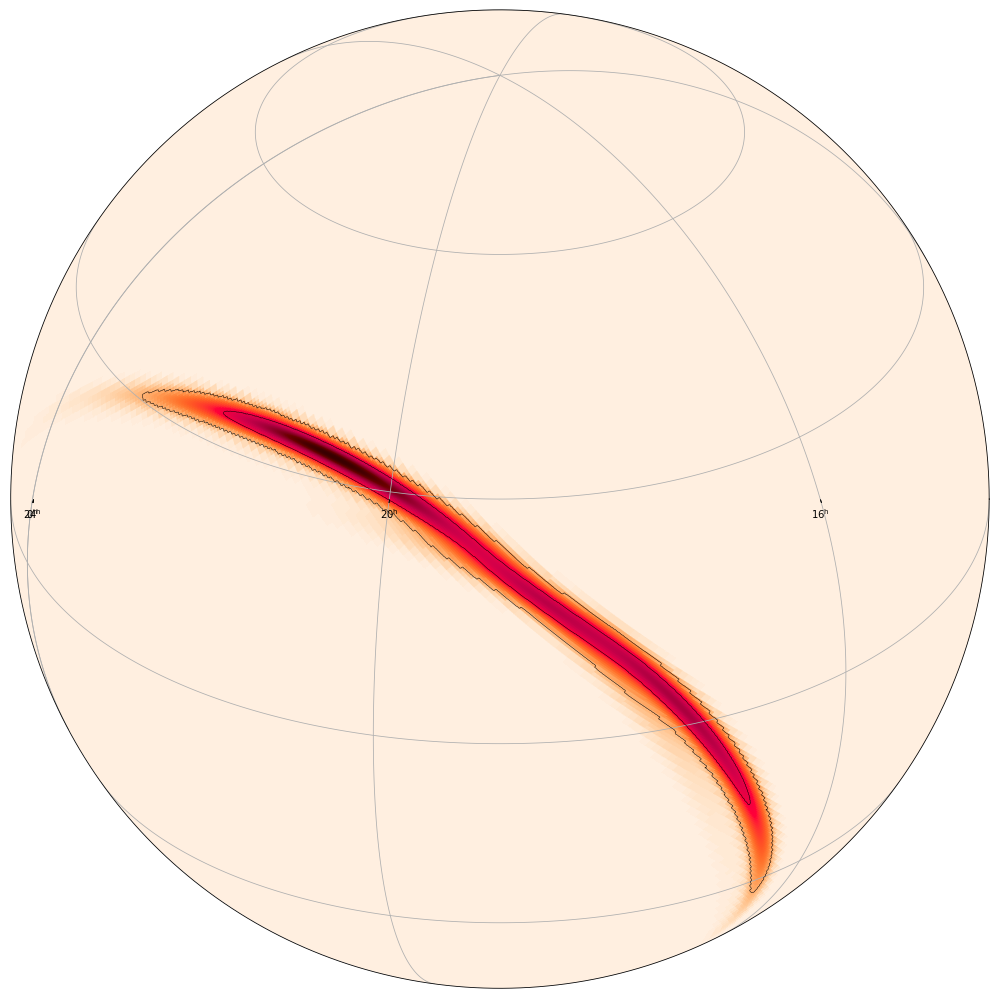
\includegraphics[width=0.5\linewidth]{images/tiling/1_0.png}} \\
            Tiles within 50\% contour: &
            Tiles within 90\% contour: \\
            47 tiles, covering 86\% &
            86 tiles, covering 98\% \\
            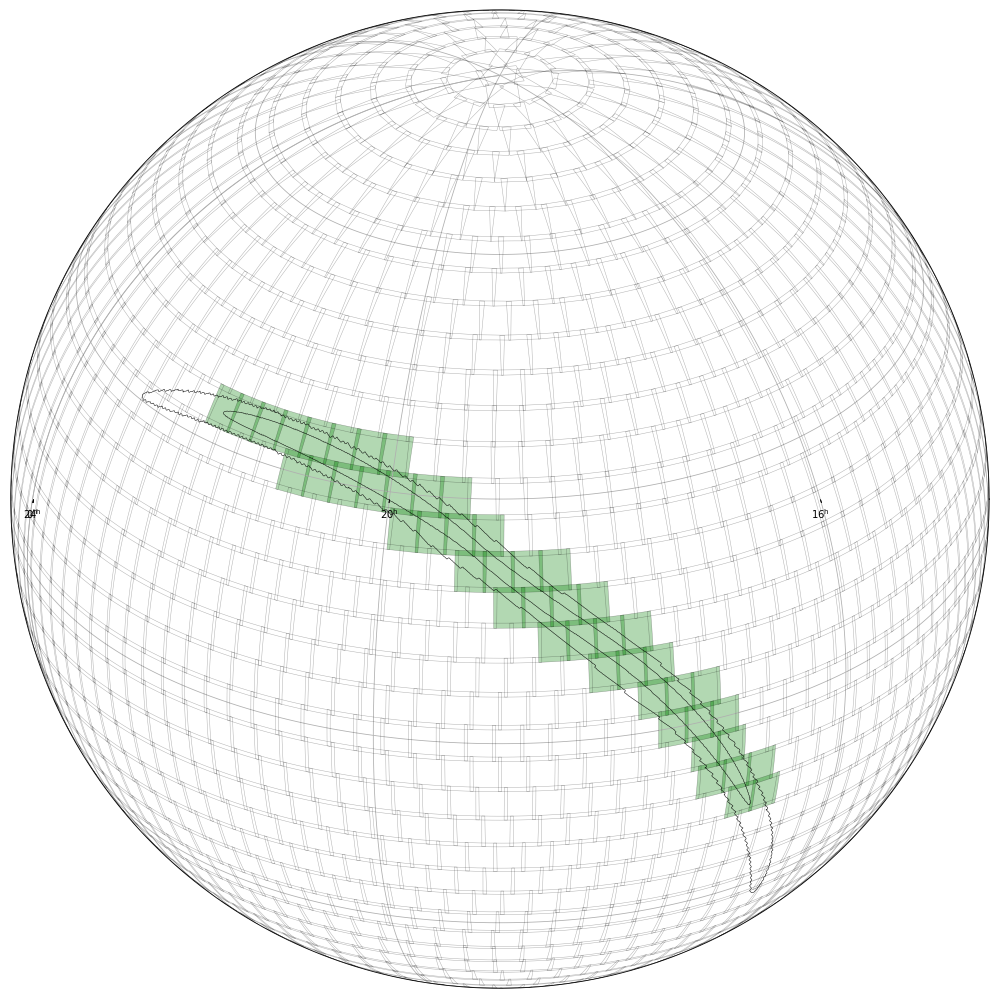
\includegraphics[width=0.25\linewidth]{images/tiling/1_c.png} &
            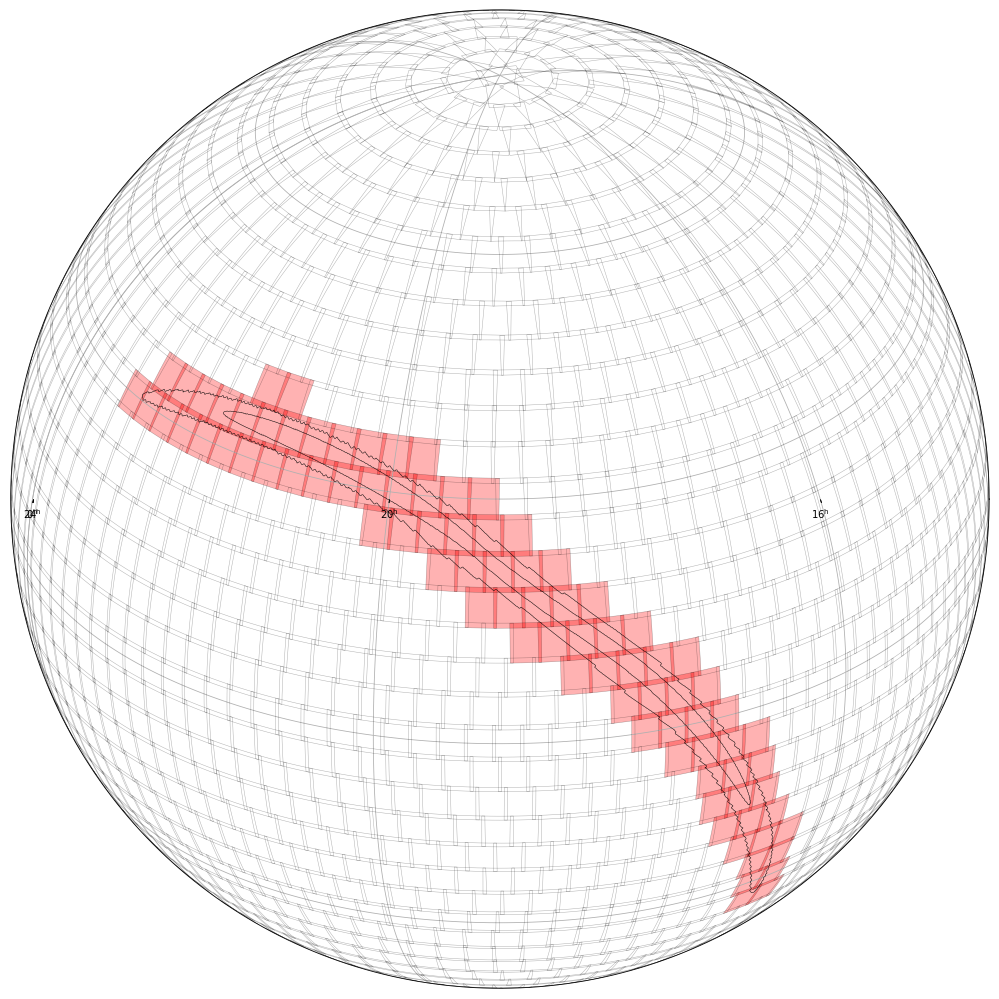
\includegraphics[width=0.25\linewidth]{images/tiling/1_d.png} \\
            Tiles with probability > 1\%: &
            Tiles with mean contour within 90\%: \\
            41 tiles, covering 90\% &
            42 tiles, covering 91\% \\
            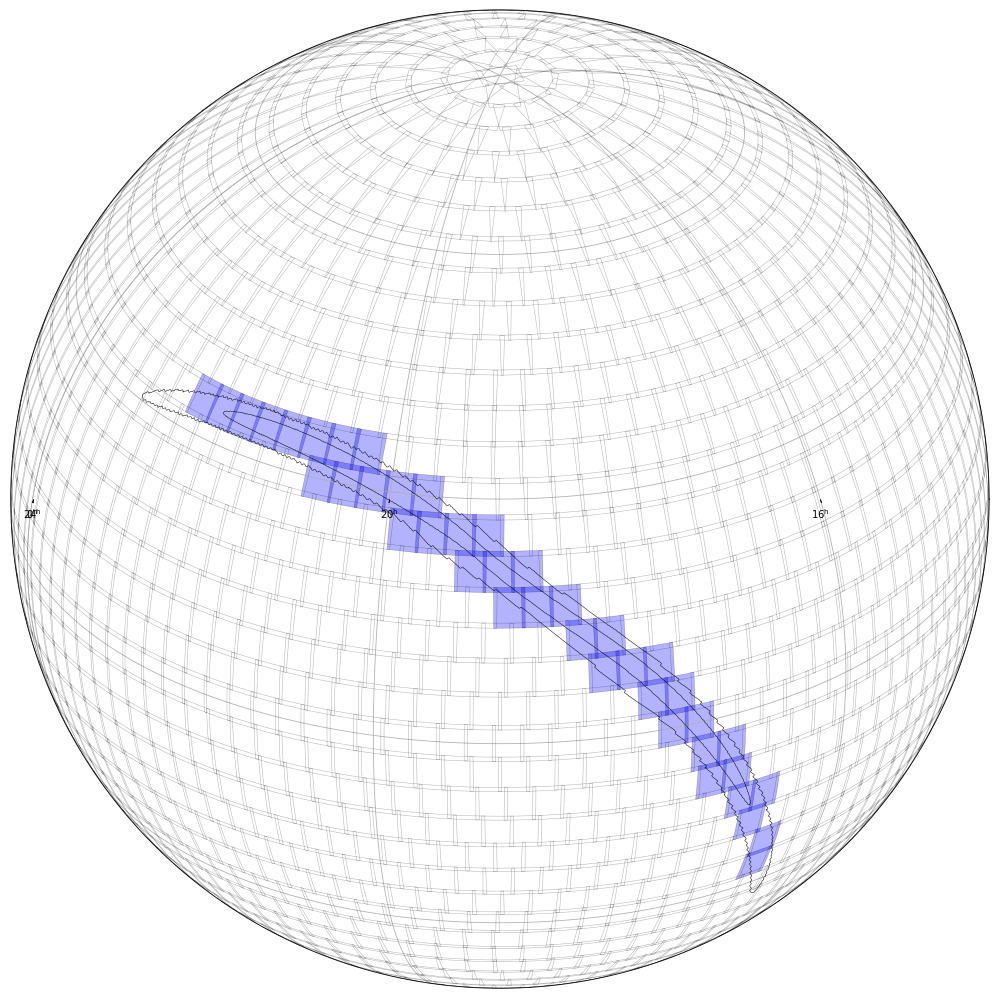
\includegraphics[width=0.25\linewidth]{images/tiling/1_a.png} &
            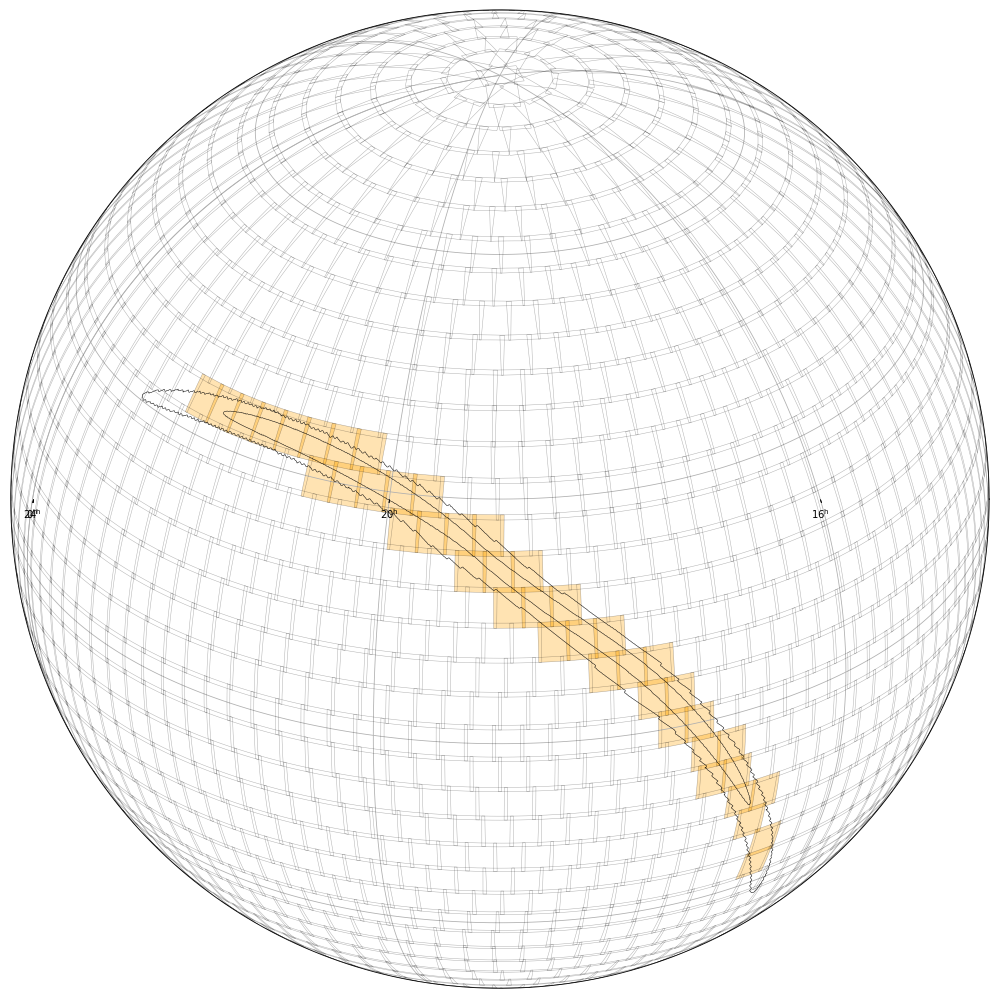
\includegraphics[width=0.25\linewidth]{images/tiling/1_b.png} \\
        \end{tabular}
    \end{center}
    \caption[Different tile selection methods for S190521r]{
        Different tile selection methods applied to the skymap for \gls{lvc} event S190521r.\\
        This is a very typical \gls{gw} skymap, and one for which the basic method of choosing tiles with a contained probability of greater than 1\% (lower-left, in blue) works well and produces almost the same set of tiles as the improved mean contour method (lower-right, in yellow). Note the inefficiencies of covering the full contours, the 50\% contour (centre-left, in green) covers less probability with more tiles than either of the lower two methods.
    }\label{fig:tiling_S190521r}
\end{figure}

\newpage

\begin{figure}[p]
    \begin{center}
        \begin{tabular}{cc}
            \multicolumn{2}{c}{Final probability skymap for event GW170817:} \\ %\todo{recolour}
            \multicolumn{2}{c}{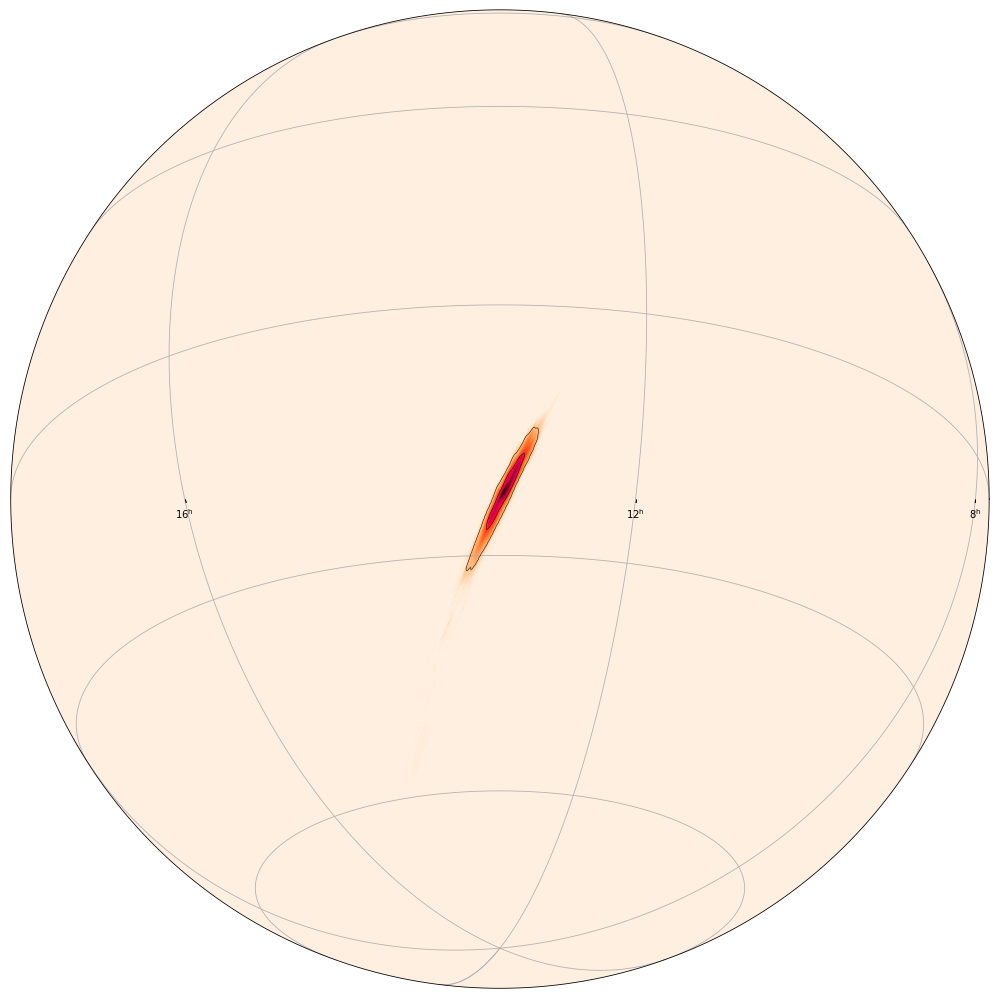
\includegraphics[width=0.5\linewidth]{images/tiling/2_0.png}} \\
            Tiles within 50\% contour: &
            Tiles within 90\% contour: \\
            6 tiles, covering 88\% &
            11 tiles, covering 96\% \\
            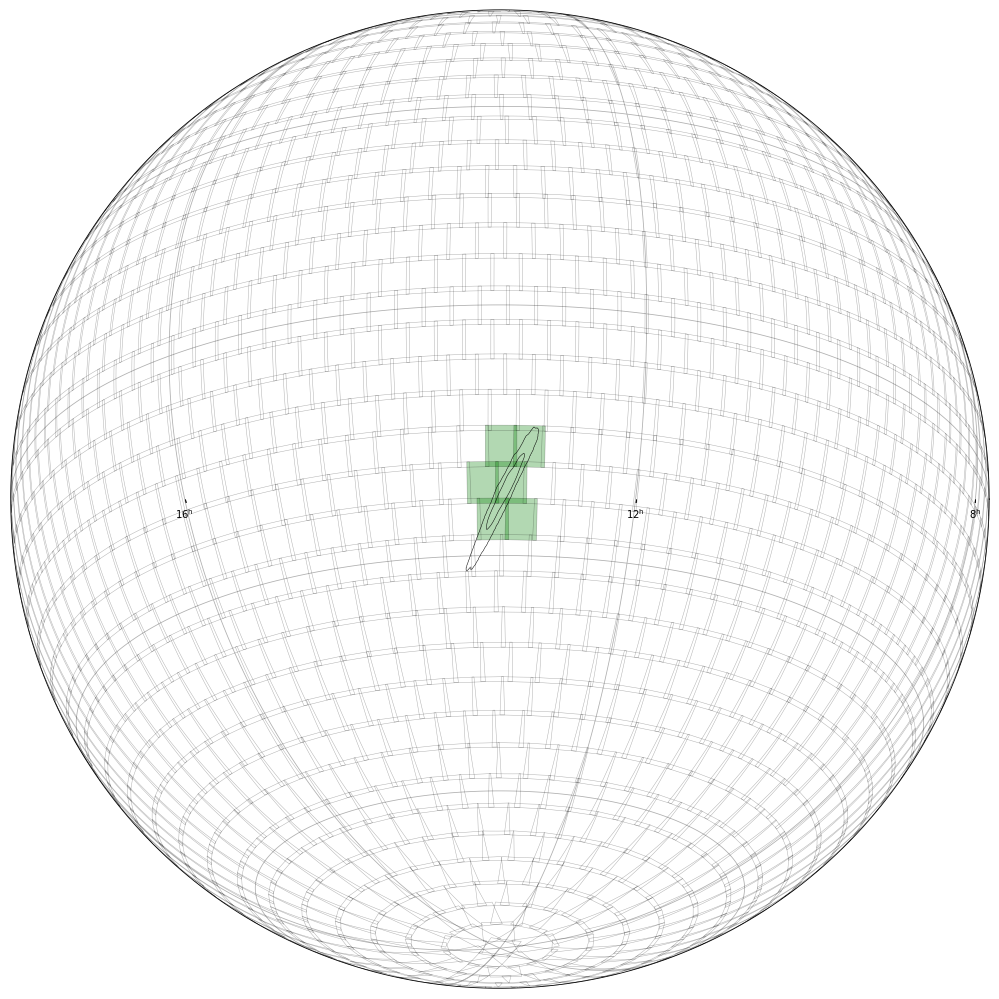
\includegraphics[width=0.25\linewidth]{images/tiling/2_c.png} &
            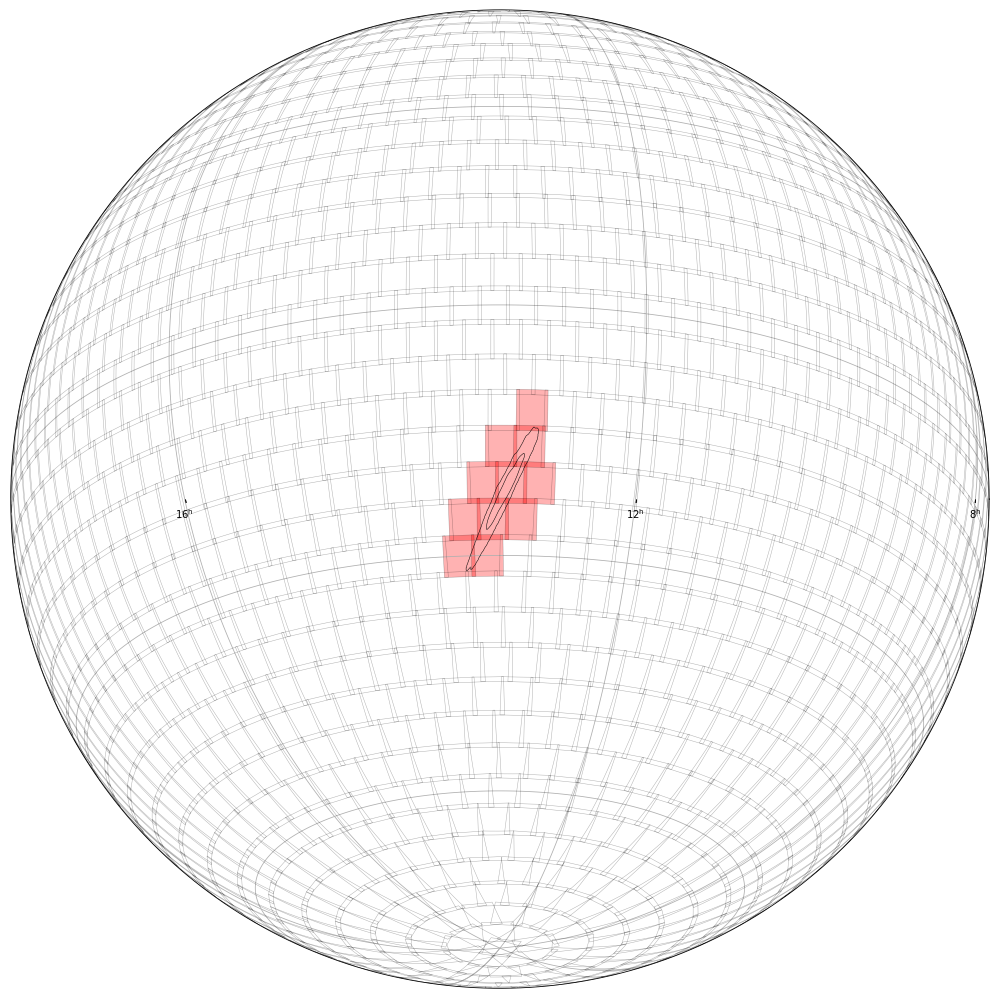
\includegraphics[width=0.25\linewidth]{images/tiling/2_d.png} \\
            Tiles with probability > 1\%: &
            Tiles with mean contour within 90\%: \\
            10 tiles, covering 98\% &
            3 tiles, covering 88\% \\
            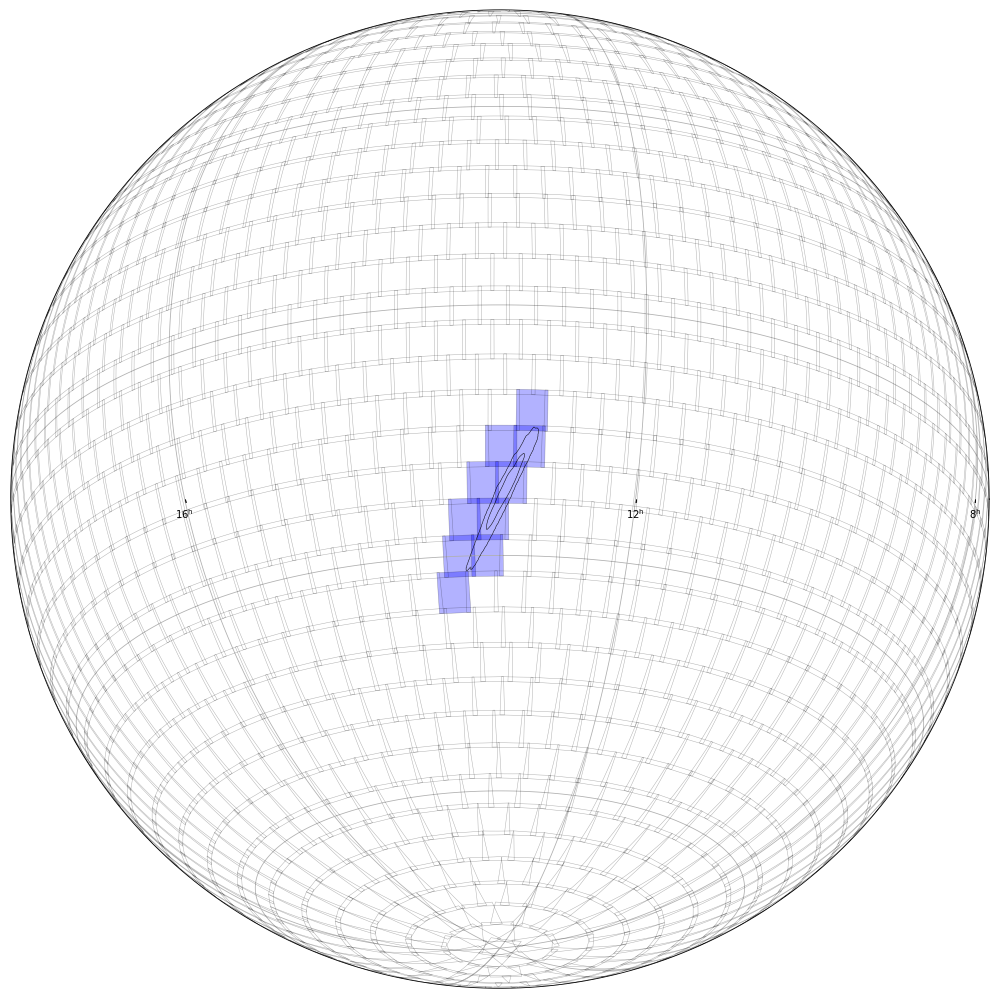
\includegraphics[width=0.25\linewidth]{images/tiling/2_a.png} &
            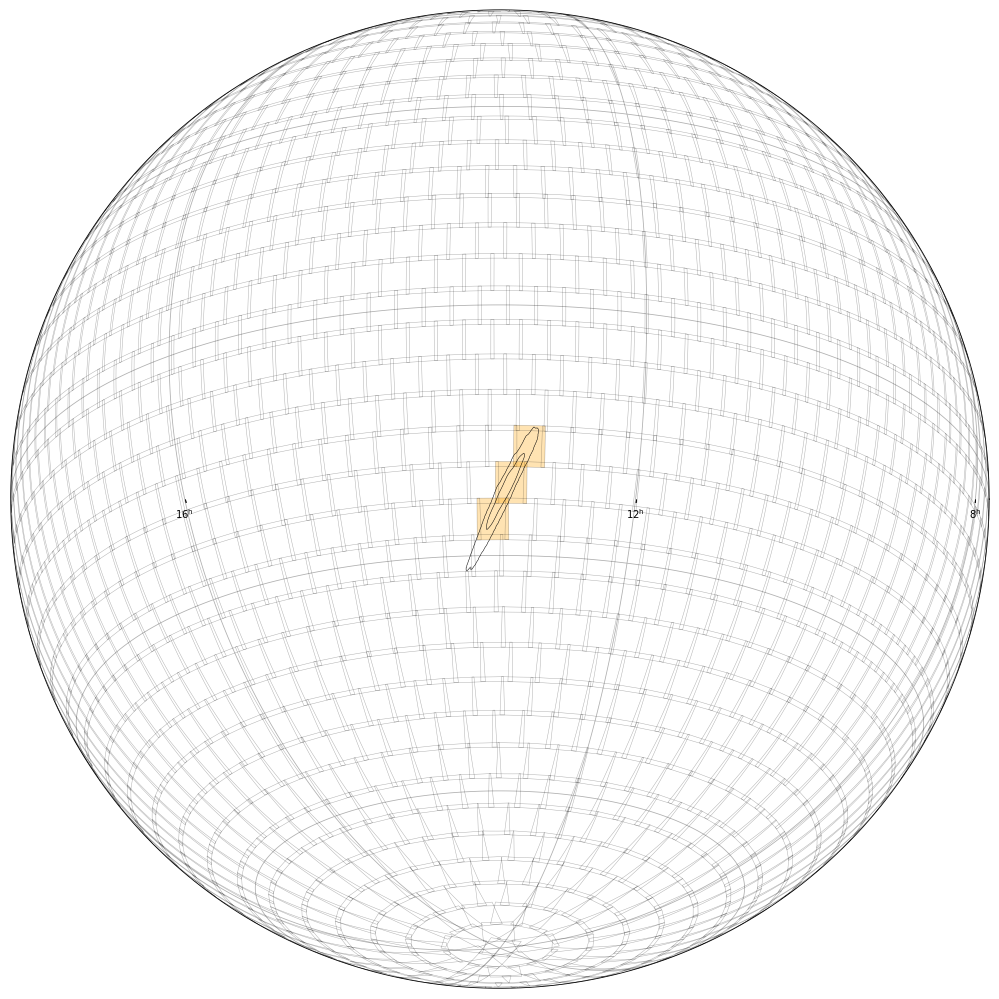
\includegraphics[width=0.25\linewidth]{images/tiling/2_b.png} \\
        \end{tabular}
    \end{center}
    \caption[Different tile selection methods for GW170817]{
        Different tile selection methods applied to the skymap for \gls{lvc} event GW170817.\\
        This skymap is atypically well localised. In this case the simple 1\% limit (lower-left, in blue) selects a large number of redundant tiles. The inefficiencies of the contour methods are also visible, the 50\% selection limit (centre-left, in green) covers the same total probability as the mean contour method (lower-right, in yellow) but with twice the number of tiles. Note the location of the actual counterpart (as shown in \aref{fig:170817_gw}) was selected by all of these methods.
    }\label{fig:tiling_GW170817}
\end{figure}

\newpage

\begin{figure}[p]
    \begin{center}
        \begin{tabular}{cc}
            \multicolumn{2}{c}{Prefered probability skymap for superevent S190425z:} \\ %\todo{recolour}
            \multicolumn{2}{c}{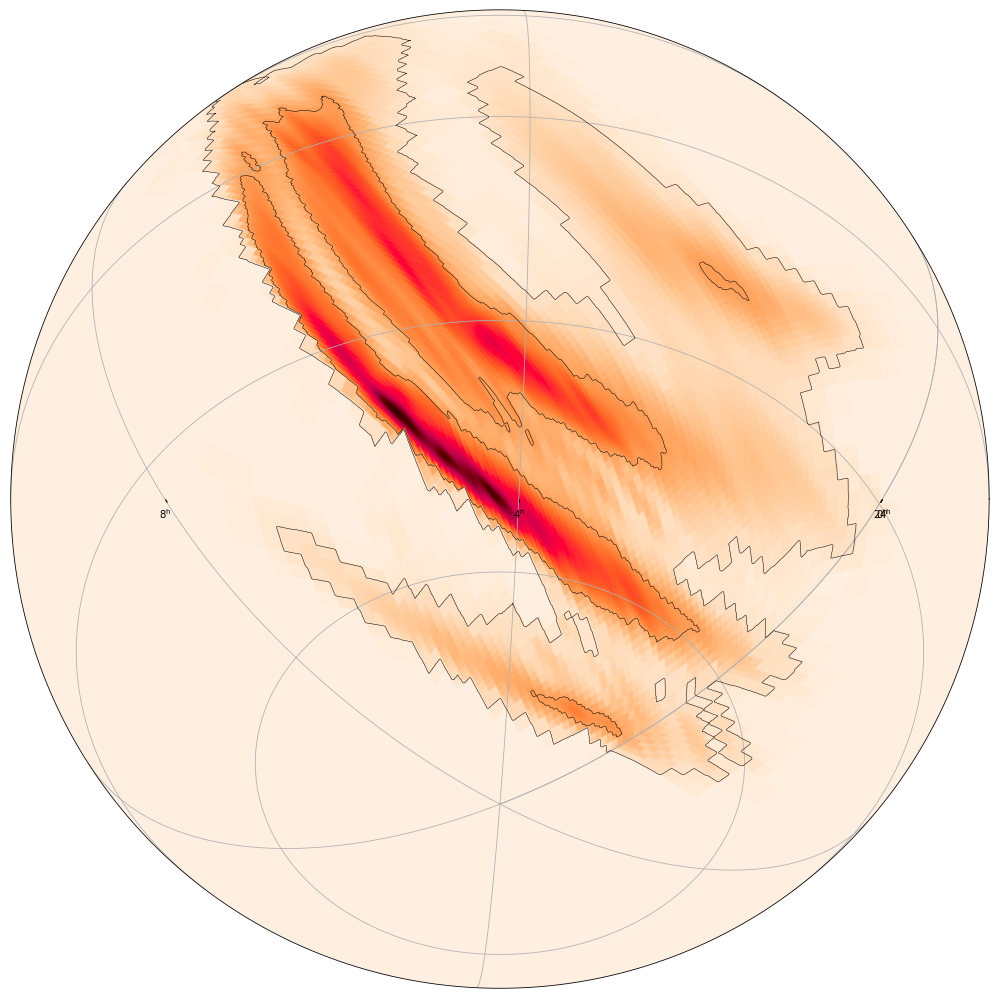
\includegraphics[width=0.5\linewidth]{images/tiling/3_0.png}} \\
            Tiles within 50\% contour: &
            Tiles within 90\% contour: \\
            207 tiles, covering 67\% &
            753 tiles, covering 95\% \\
            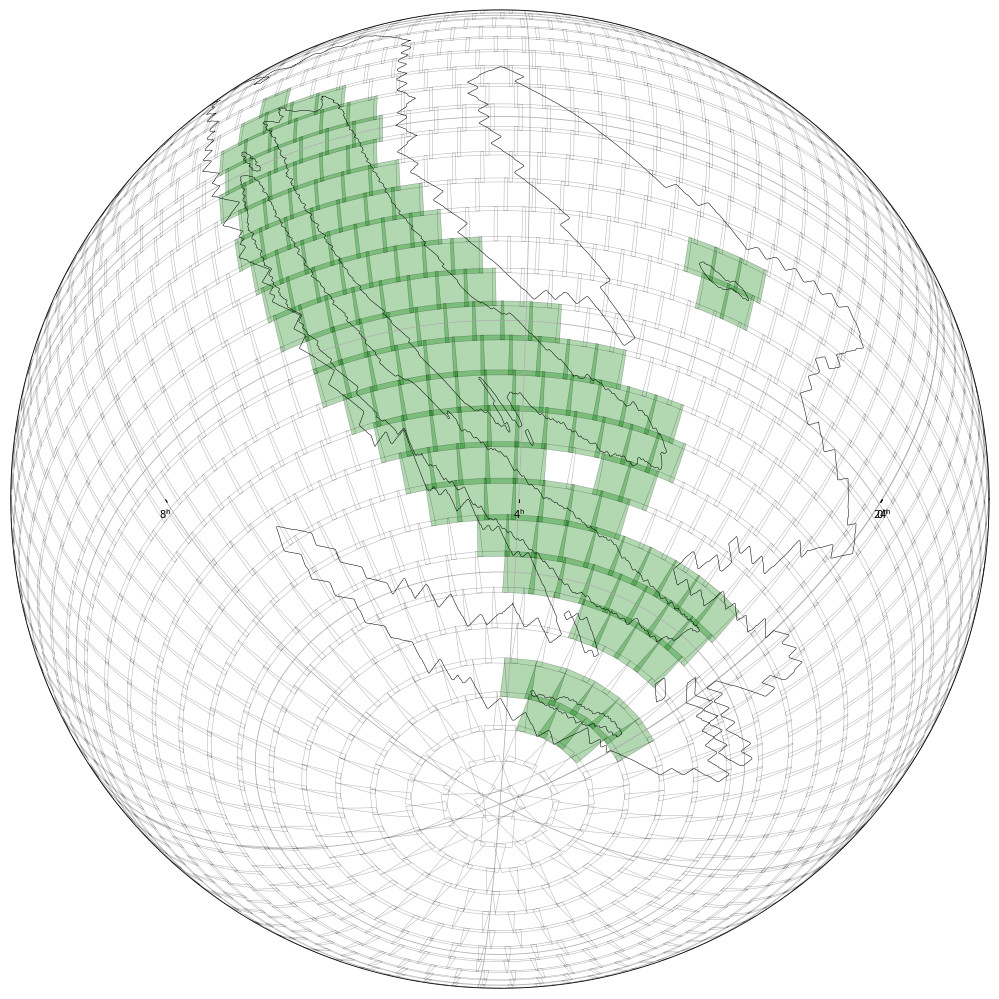
\includegraphics[width=0.25\linewidth]{images/tiling/3_c.png} &
            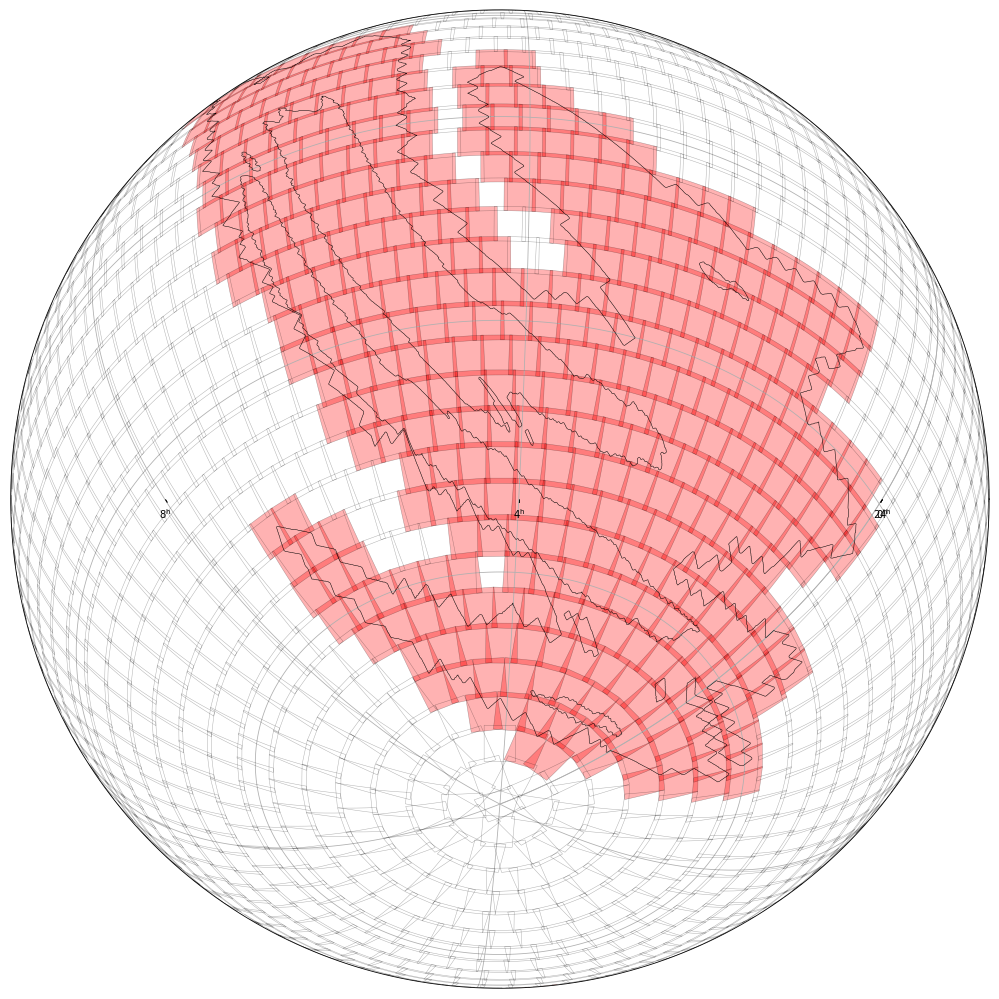
\includegraphics[width=0.25\linewidth]{images/tiling/3_d.png} \\
            Tiles with probability > 1\%: &
            Tiles with mean contour within 90\%: \\
            10 tiles, covering 11\% &
            548 tiles, covering 91\% \\
            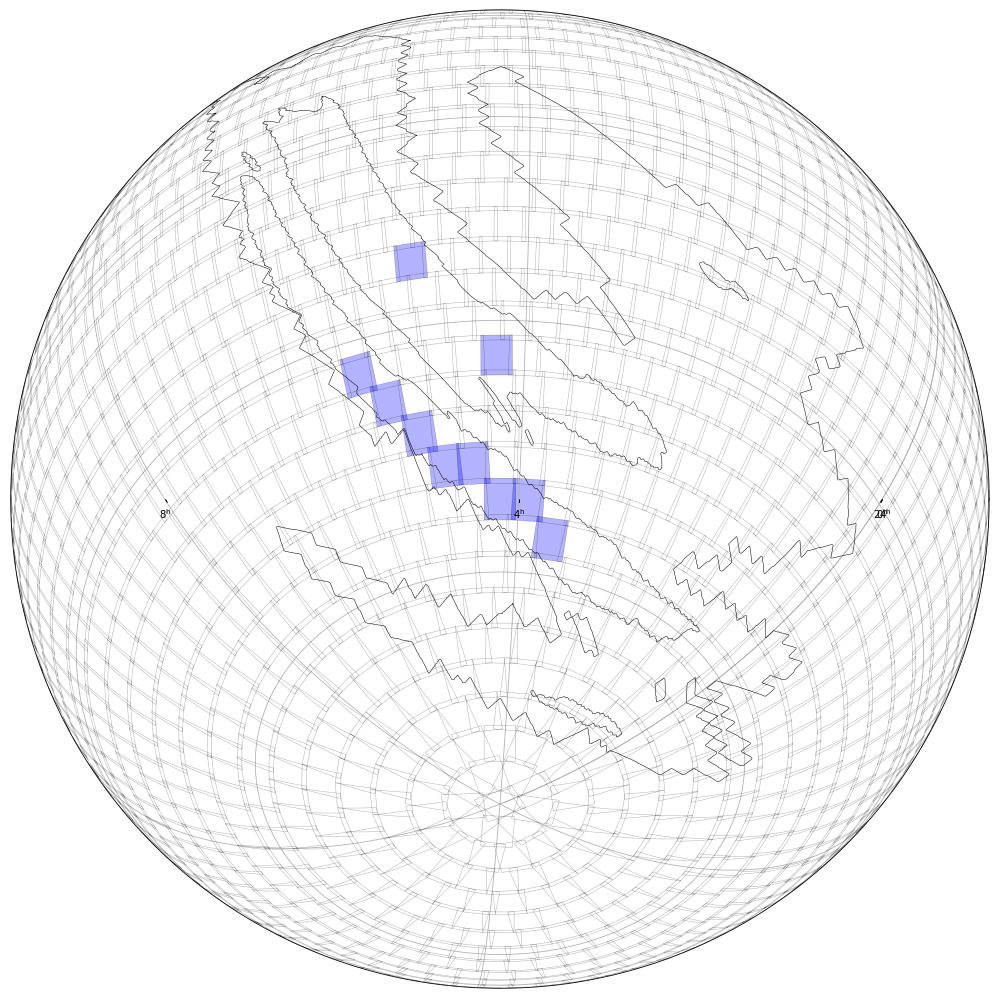
\includegraphics[width=0.25\linewidth]{images/tiling/3_a.png} &
            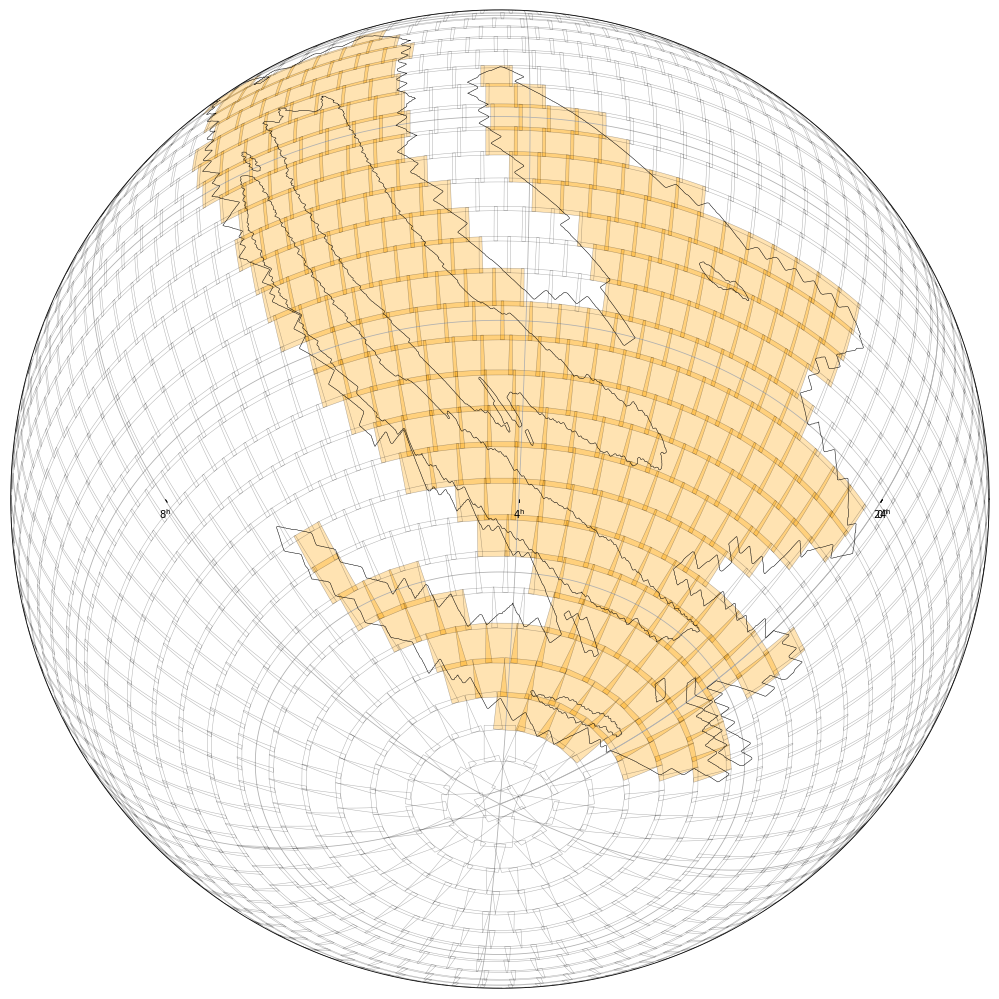
\includegraphics[width=0.25\linewidth]{images/tiling/3_b.png} \\
        \end{tabular}
    \end{center}
    \caption[Different tile selection methods for S190425z]{
        Different tile selection methods applied to the skymap for \gls{lvc} event S190425z.\\
        This is an atypically large skymap. The fixed 1\% limit (lower-left, in blue) is clearly unsuitable to be used in this case. The mean contour method (lower-right, in yellow) is a reasonable compromise between the two centre contour methods, covering just 4\% less than the full 90\% contour selection but with 205 fewer tiles. Note 548 tiles would still be too many to easily observe for the 4-UT system, so they would be limited to the top 200 sorted by probability.
    }\label{fig:tiling_S190425z}
\end{figure}

\clearpage

Once the chosen tiles have been selected then entries can be inserted into the observing database (defined in \aref{sec:obsdb}). First a new entry in the \code{events} table is added for this event, containing the source, type, ID and \gls{ivorn}. Then an entry in the \code{surveys} table is also created in order to group together all the pointings from this particular event. Although it is currently not used, the database is defined to allow multiple surveys per event. For example, there could be a quick initial survey in a wide-passband filter that prioritises possible host galaxies followed by a slower survey using the colour filters and longer exposure times that focuses on covering the skymap. But at the time of writing each event only has a single survey defined.

Finally the individual tiles are inserted as entries in the \code{mpointings} table. Each is connected to an entry in the \code{grid\_tiles} table for this particular grid, and the tile probabilities are stored as corresponding entries in the \code{survey\_tiles} table. The most important entries for the mpointings are the rank, target constraint values (minimum altitude, moon phase etc), the time block parameters (the time between pointings being valid) and the actual exposure settings (exposure time, filter, number in a set). These are found from the event strategy as described in \aref{sec:event_strategy}. Once the mpointings are defined the first pointings are also created and added to the database \code{pointings} table, to insure they become immediately valid in the queue without having to wait for the caretaker to create them.

After all of these entries are added to the database then the event has been successfully handled. When the scheduler next fetches the queue the pointings should be there ready to observe, and if they are valid the highest priority will be sent to the pilot to begin follow-up observations.

\end{colsection}

% ~~~~~~~~~~~~~~~~~~~~

\newpage
\subsection{Event reports}
\label{sec:event_slack}
\begin{colsection}

Throughout the event handling process GOTO-alert has the option of sending confirmation messages to Slack, in a similar way to the \gls{gtecs} pilot (see \aref{fig:pilot_slack}). This allows human observers to be informed of any new alerts processed by the sentinel, as well as the expected outcome of upcoming observations. The function deliberately spaces out the alerts it sends at different stages within the code, rather than sending them all at the end, to make sure it's obvious if a problem occurs and one or more alerts are missing. Four alerts are sent out in total:

\begin{enumerate}
    \item An initial alert is sent out by the sentinel as soon as an interesting event is received, and contains only one line reporting the IVORN of the event to be processed. Sending this first means there is a record should an error occur subsequently while handling the event.
    \item The first alert is sent out by GOTO-alert once the event has been created and the skymap downloaded. It contains the key information and properties of the event, as well as a plot of the event skymap produced by GOTO-tile.
    \item The next alert is sent out after the event observing strategy has been retrieved, and reports the contents of the strategy dictionaries (see \aref{sec:event_strategy}).
    \item The final alert is sent out after the event tiles have been added to the observation database (see \aref{sec:event_insert}). As well as showing the number of tiles selected and their combined skymap coverage this alert also contains predictions of which tiles will be visible from the GOTO site in La Palma over the valid period. Ultimately this could also include a second corresponding calculation of visibility from GOTO-South as well. Note this is only a rough prediction based on visible altitudes during the night, and therefore excluding weather conditions, the position of the Moon and the existence of any higher-priority pointings that would take precedence (see \aref{sec:scheduler} for how the \gls{gtecs} just-in-time scheduler operates).
\end{enumerate}

The three detailed alerts generated by GOTO-alert for an example \gls{gw} event are shown in \aref{fig:pilot_slack}.

Should a retraction notice be received for an event previously processed by the sentinel then strategy and visibility alerts would not be applicable. Instead once it has been handled a special alert will be sent out, clarifying that the retraction was received and any previously-inserted pointings have been deleted.

\begin{sidewaysfigure}[p]
    \begin{center}
        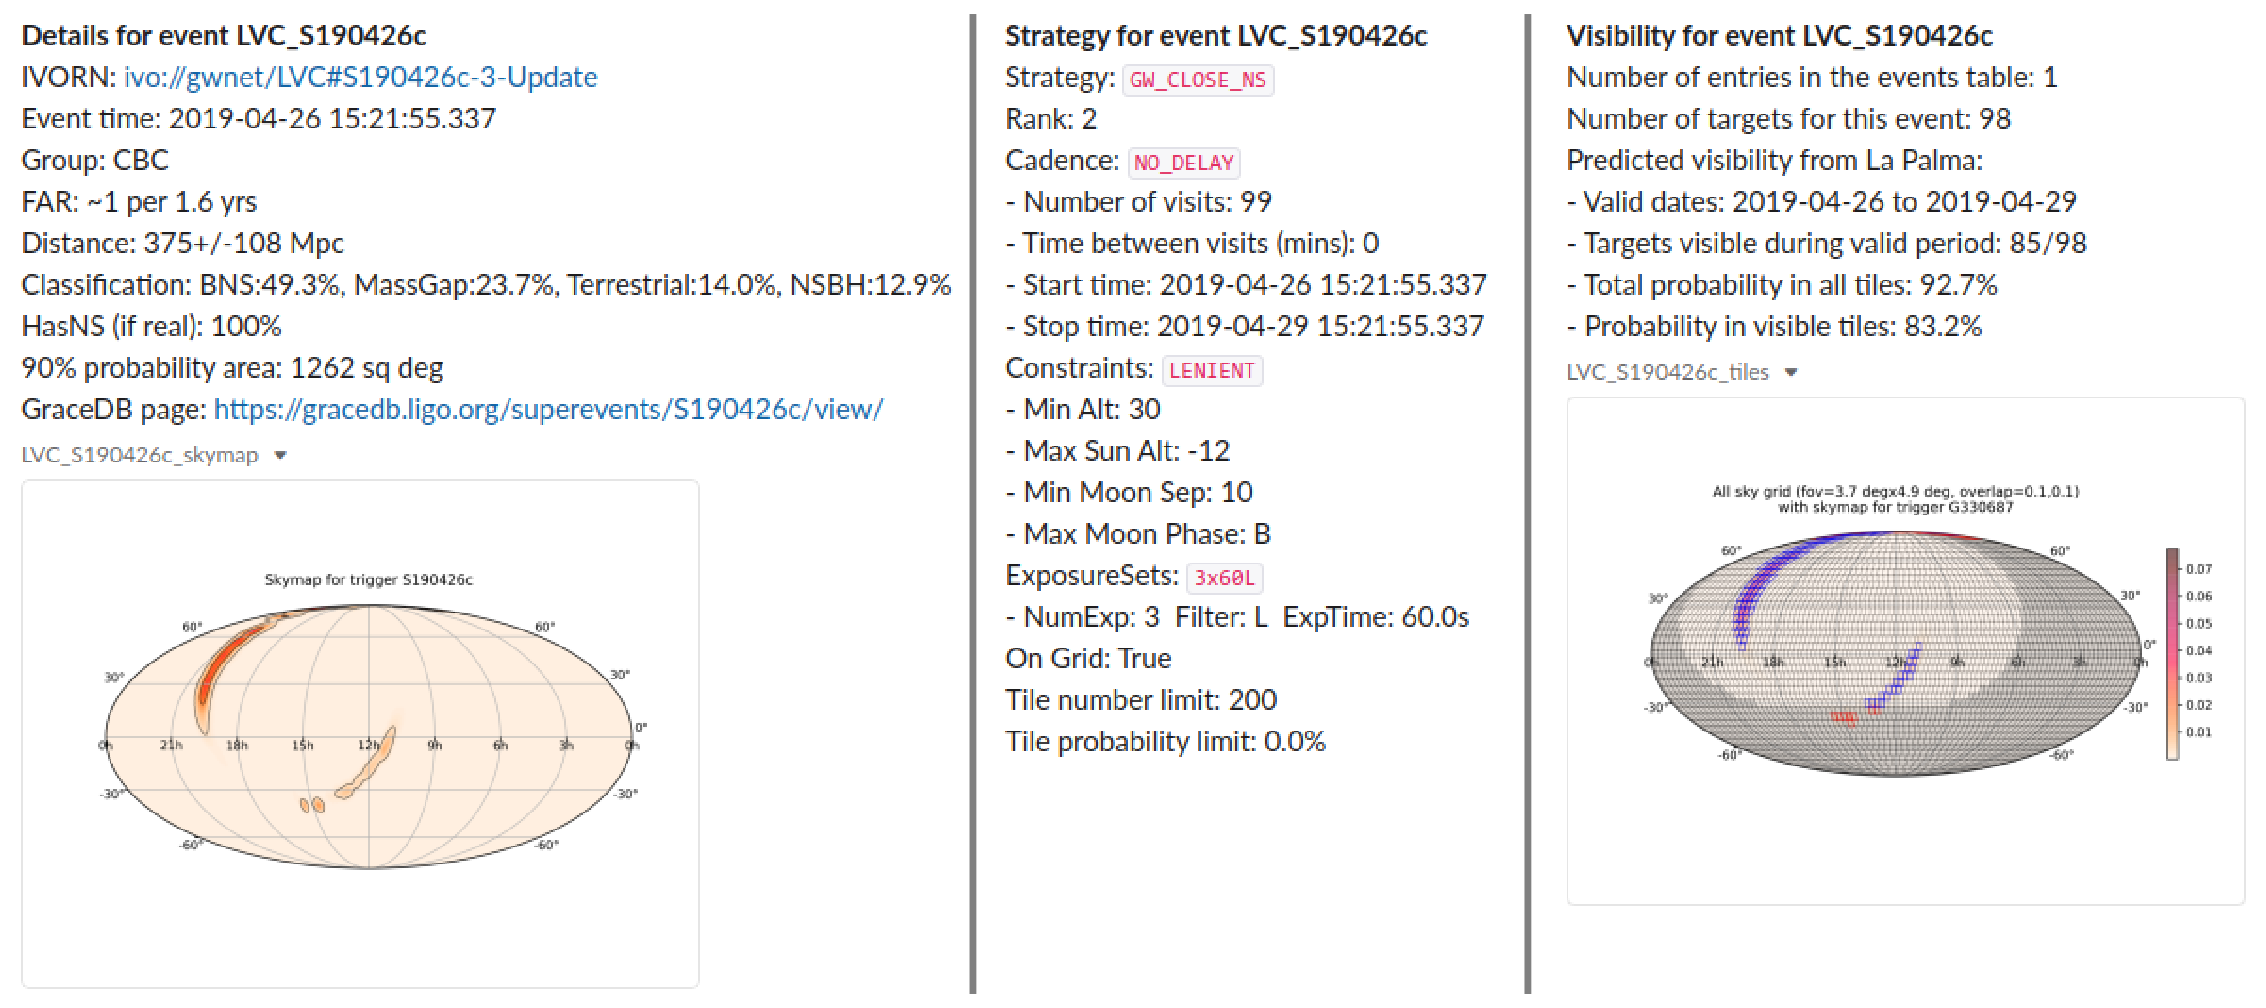
\includegraphics[width=\linewidth]{images/gototile_slack_side.png} %\todo{redo with GOTObot?}
    \end{center}
    \caption[Slack alerts created by GOTO-tile for a GW event]{
        Slack alerts generated by the GOTO-tile event handler for a real gravitational wave event, S190426c.\\
        \textbf{Left}: The first alert includes key information about the event gathered from the GCN notice, for \gls{gw} events that includes \gls{far}, classification and distance information, a link to the GraceDB entry and a skymap image generated by GOTO-tile.\\
        \textbf{Centre}: The second alert details the event observing strategy (see \aref{sec:event_strategy}).\\
        \textbf{Right}: The third alert gives the consequences of the applied strategy: the number of tiles inserted into the database and their visibility over the valid period. The attached GOTO-tile plot shows a prediction of which tiles covering the skymap will be visible.
    }\label{fig:gototile_slack}
\end{sidewaysfigure}

\end{colsection}

% ~~~~~~~~~~~~~~~~~~~~

\end{colsection}

% ########################################
